\subsection{小さい圏の圏}
	関手は圏から圏への一種の写像であるため、集合の圏のように、圏を対象とし関手を射とするような圏である圏の圏を考えることができそうである。
	そのためにもまずは合成射、恒等射にあたる関手を定義していく。
	\begin{define}[合成関手]
		関手$\functor{F}{C}{C'}$、$\functor{G}{C'}{C''}$を合成した関手$\functor{G\circ F}{C}{C'}$を以下の要素によって定義する。
		\begin{quote}
			\begin{mydescription}
			\item[対象関数]関手$F,G$のそれぞれの対象関数$F,G$に対して$G\circ F$の対象関数を$G\circ F$と定義する。つまり圏$\cat{C}$の任意の対象$A$に対して\[(G\circ F)(A)=G(FA)\]となるような写像である。
			\item[射関数]関手$F,G$のそれぞれの射関数$F,G$に対して$G\circ F$の射関数を$G\circ F$と定義する。
			つまり圏$\cat{C}$の任意の対象$A,A'$と任意の射$\mor{f}{A}{A'}$に対して\[\mor{(G\circ F)_{}(f)=G(Ff)}{GFA}{GF{A'}}\]となるような写像である。

			各二対象ごとの射関数も見ていくと、関手$F,G$のそれぞれの関数\[\mor{F_{A,A'}}{\arset{C}{A}{A'}}{\arset{C'}{FA}{FA'}}\]\[\mor{G_{FA,FA'}}{\arset{C'}{FA}{FA'}}{\arset{C''}{GFA}{GFA'}}\]に対して$G\circ F$の関数を\[(G\circ F)_{A,A'}=\mor{G_{FA,FA'}\circ F_{A,A'}}{\arset{C}{A}{A'}}{\arset{C''}{GFA}{GFA'}}\]となる。このように関手の合成はそれぞれの関手の対象関数、射関数の合成に還元して考える。

			\begin{center}
				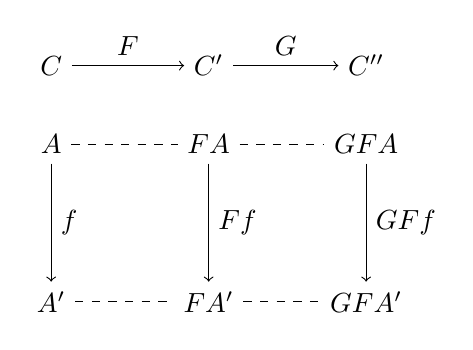
\begin{tikzpicture}[auto]
					\node (a) at (0, 2) {$A$};
					\node (a') at (0, 0) {$A'$};
					\node (fa) at (2, 2) {$FA$};
					\node (fa') at (2, 0) {$FA'$};
					\node (gfa) at (4, 2) {$GFA$};
					\node (gfa') at (4, 0) {$GFA'$};
					\node (catc) at (0, 3) {$\cat{C}$};
					\node (catc') at (2, 3) {$\cat{C'}$};
					\node (catc'') at (4, 3) {$\cat{C''}$};
					\draw[-,dashed] (a) to (fa);
					\draw[-,dashed] (a') to (fa');
					\draw[-,dashed] (fa) to (gfa);
					\draw[-,dashed] (fa') to (gfa');
					\draw[->] (catc) to node{$F$}(catc');
					\draw[->] (catc') to node{$G$}(catc'');

					\draw[->] (a) to node{$f$}(a');
					\draw[->] (fa) to node{$Ff$}(fa');
					\draw[->] (gfa) to node{$GFf$}(gfa');

				\end{tikzpicture}
			\end{center}
			また紛らわしくない場合は合成関手$G\circ F$を$GF$と略すことにする。
			\item[恒等射の保存] $GF(id_A)=id_{GFA}$を示せばよい。
				\begin{align*}
					GF(id_A)&=G(F(id_A))&\text{(射関数の定義)}\\
					&=G(id_{FA})&\text{(関手$F$の恒等射の保存)}\\
					&=id_{GFA}&\text{(関手$G$の恒等射の保存)}
				\end{align*}
			よって合成関手は恒等射を保つ。
			\item[射の合成の保存] $GF(g\circ f)=GFg\circ GFf$を示せばよい。
				\begin{align*}
					GF(g\circ f)&=G(F(g\circ f))&\text{(射関数の定義)}\\
					&=G(Fg\circ Ff)&\text{(関手$F$の射の合成の保存)}\\
					&=GFg\circ GFf&\text{(関手$G$の射の合成の保存)}
				\end{align*}
			よって合成関手は射の合成を保つ。
			\begin{center}
				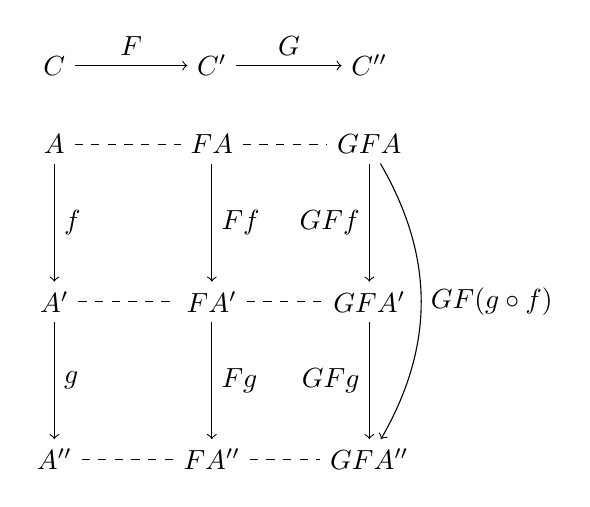
\begin{tikzpicture}[auto]
					\node (a) at (0, 2) {$A$};
					\node (a') at (0, 0) {$A'$};
					\node (a'') at (0, -2) {$A''$};
					\node (fa) at (2, 2) {$FA$};
					\node (fa') at (2, 0) {$FA'$};
					\node (fa'') at (2, -2) {$FA''$};
					\node (gfa) at (4, 2) {$GFA$};
					\node (gfa') at (4, 0) {$GFA'$};
					\node (gfa'') at (4, -2) {$GFA''$};
					\node (catc) at (0, 3) {$\cat{C}$};
					\node (catc') at (2, 3) {$\cat{C'}$};
					\node (catc'') at (4, 3) {$\cat{C''}$};
					\draw[-,dashed] (a) to (fa);
					\draw[-,dashed] (a') to (fa');
					\draw[-,dashed] (a'') to (fa'');
					\draw[-,dashed] (fa) to (gfa);
					\draw[-,dashed] (fa') to (gfa');
					\draw[-,dashed] (fa'') to (gfa'');
					\draw[->] (catc) to node{$F$}(catc');
					\draw[->] (catc') to node{$G$}(catc'');

					\draw[->] (a) to node{$f$}(a');
					\draw[->] (a') to node{$g$}(a'');

					\draw[->] (fa) to node{$Ff$}(fa');
					\draw[->] (fa') to node{$Fg$}(fa'');

					\draw[->] (gfa) to node[swap]{$GFf$}(gfa');
					\draw[->] (gfa') to node[swap]{$GFg$}(gfa'');
					\draw[->,bend left =30] (gfa) to node{$GF(g\circ f)$}(gfa'');
				\end{tikzpicture}
			\end{center}
		\end{mydescription}
		\end{quote}
	\end{define}
	\begin{define}[恒等関手]
		任意の圏$\cat{C}$の\textbf{恒等関手}$\functor{Id_{\cat{C}}}{C}{C}$を以下の要素で定義する。
		\begin{quote}
			\begin{mydescription}
				\item[対象関数] 対象関数を恒等写像$Id_{\cat{C}}(A)=A$と定義する。
				\item[射関数] 射関数を恒等写像$Id_{\cat{C}}(f)=f$と定義する。
				\item[恒等射の保存] $Id_{\cat{C}}(id_C)=id_C=id_{Id_{\cat{C}}(C)}$より恒等射を保つ
				\item[射の合成の保存] $Id_{\cat{C}}(g\circ f)=g\circ f=Id_{\cat{C}}(g)\circ Id_{\cat{C}}(f)$より射の合成を保つ。
			\end{mydescription}
		\end{quote}
	\end{define}
	\begin{define}[小さい圏の圏]
		\textbf{小さい圏の圏}$\cat{Cat}$は以下の要素で構成される。

		集合の圏の時と同様に、小さい圏の「小さい」とは簡単に説明をするのであれば自己言及を防ぐための条件付けであり、実際に$\cat{Cat}$は小さい圏ではないため$\cat{Cat}$の対象にはならない。
		\begin{quote}
			\begin{mydescription}
				\item[対象] 任意の小さい圏
				\item[射] 任意の小さい圏$\cat{A,B}$の間の任意の関手$\functor{F}{A}{B}$
				\item[射の合成] 関手$\functor{F}{C}{C'}$、$\functor{G}{C'}{C''}$に対して合成した関手$\functor{G\circ F}{C}{C'}$をとる操作を射の合成とする。
				\item[恒等射の存在]任意の圏$\cat{A}$の恒等関手$Id_{\cat{A}}$を恒等射とする。
				\item[結合律]
				$H\circ (G\circ F)=(H\circ G)\circ F$が合成可能な任意の関手$F,G,H$で成り立つことを示せばよい。
				二つの関手が等しいことを示すにはそれぞれを構成する対象関数と射関数が等しいことを示せばよい。
				対象関数については、関手$F,G,H$の対象関数$F,G,H$に対して$H\circ (G\circ F)=(H\circ G)\circ F$は明らかに成り立つ。
				射関数についても写像の結合律に還元すると、
				\begin{align*}
					(H\circ (G\circ F))_{A,A'}&=H_{GFA,GFA'}\circ (G\circ F)_{A,A}&\text{(射関数の合成の定義)}\\
					&=H_{GFA,GFA'}\circ (G_{FA,FA'}\circ F_{A,A'})&\text{(射関数の合成の定義)}\\
					&=(H_{GFA,GFA'}\circ G_{FA,FA'})\circ F_{A,A'}&\text{(写像の結合則)}\\
					&=(H\circ G)_{FA,FA'}\circ F_{A,A'}&\text{(射関数の合成の定義)}\\
					&=(H\circ (G\circ F))_{A,A'}&\text{(射関数の合成の定義)}
				\end{align*}
				となり、射関数においても結合則が成り立つ。
				\item[単位元律]
				任意の圏$\cat{C}$の恒等関手$Id_{\cat{C}}$と任意の関手$\functor{F}{X}{C}$、$\functor{G}{C}{Y}$において$Id_{\cat{C}}\circ F=F$、$G\circ Id_{\cat{C}}=G$が成り立つことを示せばよい。

				恒等関手の対象関数、射関数ともに恒等写像
				\[\mor{Id_\cat{C}=id_{\obj{A}}}{\obj{A}}{\obj{A}}\]
				\[\mor{Id_{\cat{C}A,A'}=id_{\arset{C}{A}{A'}}}{\arset{C}{A}{A'}}{\arset{C}{A}{A'}}\]
				となるため、写像の単位元律より$Id_{\cat{C}}\circ F=F$、$G\circ Id_{\cat{C}}=G$が成り立ち単位元律が成り立つ。
			\end{mydescription}
		\end{quote}
	\end{define}